\documentclass[11pt,a4paper]{article}
\usepackage[utf8]{inputenc}
\usepackage[margin=22mm]{geometry}
\usepackage{amsmath,amssymb}
\usepackage{booktabs}
\usepackage{graphicx}
\usepackage{tikz}
\usetikzlibrary{arrows.meta,positioning,calc}
\usepackage[hidelinks]{hyperref}
\usepackage{caption}
\captionsetup{font=small}

\newcommand{\Vdo}{V_{d0}}
\newcommand{\Id}{I_d}
\newcommand{\ex}{e_x}
\newcommand{\dx}{d_x}
\newcommand{\Ell}{E_{2}}

\title{Sizing of a 16.4\,V / 1100\,A six-pulse thyristor rectifier\\
\large 400\,V line (360--440\,V), transformer, line reactor with 5th/7th/11th traps, DC LC filter}
\author{Davide Bagnara}
\date{September 2026}

\begin{document}
\maketitle

\begin{abstract}
This note sizes a single fully-controlled six-pulse thyristor bridge that must deliver 16.4\,V at 1100\,A into a resistive load from a 400\,V line that may be as low as 360\,V. The chain is: 400\,V bus, series line reactor, tuned traps for the 5th, 7th and 11th harmonics, converter transformer, bridge, DC LC filter, load. The central result is the transformer secondary voltage: 17\,V rms line-to-line at 400\,V primary (15.2\,V at 360\,V, ratio 23.5), which gives a firing angle of $12^\circ$ at 360\,V, $28^\circ$ at 400\,V and $36^\circ$ at 440\,V. The transformer leakage inductance (2.1\,$\mu$H per phase on the secondary, 1.2\,mH on the primary) and winding resistance (0.29\,m$\Omega$ per phase referred to the secondary, 0.25\,$\Omega$ per primary delta phase) are estimated and their voltage drops included. The reactive demand never exceeds 17\,kvar, the 11\,kvar of the traps cover it, the current THD at the point of common coupling is below 4\,\% referred to the converter's own 36\,A fundamental, and the load voltage ripple is below 2\,\% peak-to-peak with a 0.3\,mH / 5\,mF DC filter. The general relations and the design choices follow the companion note on the multi-voltage 1\,MW supply \cite{acdc}, of which this unit is the 1-unit (B1) bridge.
\end{abstract}

\tableofcontents

\section{Scope and data}

\begin{figure}[h]
\centering
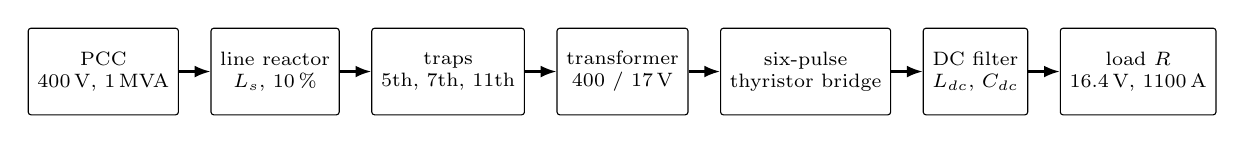
\begin{tikzpicture}[node distance=4mm,
  blk/.style={draw, rounded corners=1pt, minimum height=11mm, minimum width=13mm, align=center, font=\scriptsize},
  arr/.style={-{Latex[length=2mm]}, thick}]
\node[blk] (pcc) {PCC\\400\,V, 1\,MVA};
\node[blk, right=of pcc] (ls) {line reactor\\$L_s$, 10\,\%};
\node[blk, right=of ls] (fl) {traps\\5th, 7th, 11th};
\node[blk, right=of fl] (tr) {transformer\\400 / 17\,V};
\node[blk, right=of tr] (br) {six-pulse\\thyristor bridge};
\node[blk, right=of br] (dc) {DC filter\\$L_{dc}$, $C_{dc}$};
\node[blk, right=of dc] (ld) {load $R$\\16.4\,V, 1100\,A};
\draw[arr] (pcc) -- (ls); \draw[arr] (ls) -- (fl); \draw[arr] (fl) -- (tr);
\draw[arr] (tr) -- (br); \draw[arr] (br) -- (dc); \draw[arr] (dc) -- (ld);
\end{tikzpicture}
\caption{Power chain. The traps sit on the converter side of the line reactor, so that the reactor is between the filter bus and the grid.}
\label{fig:chain}
\end{figure}

\begin{itemize}
\item Line: 400\,V, 50\,Hz, three-phase, $\pm10$\,\% (360--440\,V). Connection rated $S_n = 1$\,MVA, fed by an MV/LV transformer with $u_k = 6$\,\% (assumed): $S_{sc} \approx 16.7$\,MVA, $X_S = 9.6$\,m$\Omega$ at 400\,V.
\item Load: resistive, $V_{out} = 16.4$\,V, $I_d = 1050$\,A in service, 1100\,A rated; $R = 14.9$\,m$\Omega$. Power 17--18\,kW.
\item Targets: line-current THD $\le 5$\,\% at the PCC referred to the converter's own fundamental (the conservative reading; IEC\,61000-3-12 and IEEE\,519 refer harmonics to the rated or maximum demand current of the connection, 1443\,A here, against which this unit is invisible); load voltage ripple $\le 5$\,\% peak-to-peak; firing angle low enough that no reactive compensation beyond the traps is needed.
\item Bridge data: relative commutation reactance $\ex = 6$\,\% and relative resistive drop $e_r = 2.7$\,\% on the secondary rating (transformer plus wiring, Section~\ref{sec:lr}), thyristor on-state drop $V_T = 1.3$\,V (two in series), minimum firing angle $\alpha_{min} = 10^\circ$ at the lowest line voltage and rated current.
\end{itemize}

\section{Relations}

For a six-pulse bridge with smooth DC current, secondary line-to-line voltage $\Ell$ and firing angle $\alpha$ \cite{iec60146,kimbark}:
\begin{align}
\Vdo &= \frac{3\sqrt2}{\pi}\Ell = 1.35\,\Ell, \qquad
V_d = \Vdo\cos\alpha - \dx - d_r - 2V_T, \label{eq:vd}\\
\dx &= \frac{\ex}{2}\Vdo\frac{\Id}{\Id{}_{,r}}, \qquad d_r = e_r\Vdo\frac{\Id}{\Id{}_{,r}}, \nonumber\\
\cos\alpha - \cos(\alpha+u) &= \frac{2\dx}{\Vdo}, \qquad
I_2 = 0.816\,\Id, \qquad I_1 = 0.78\,\Id, \qquad S_1 = \Vdo\Id, \label{eq:s1}\\
\cos\varphi_1 &\simeq \frac{\cos\alpha + \cos(\alpha+u)}{2}, \qquad P \simeq V_d\Id, \qquad Q = S_1\sin\varphi_1, \label{eq:pq}\\
\frac{I_h}{I_1} &= \frac{1}{h}\frac{\sqrt{A^2+B^2-2AB\cos(2\alpha+u)}}{\cos\alpha-\cos(\alpha+u)},\qquad h = 6k\pm1, \label{eq:harm}\\
A &= \frac{\sin\frac{(h-1)u}{2}}{h-1},\qquad B = \frac{\sin\frac{(h+1)u}{2}}{h+1}, \nonumber\\
\frac{V_n}{\Vdo} &= \frac{\sqrt2}{n^2-1}\sqrt{1+(n^2-1)\sin^2\alpha}, \quad n = 6k \quad\text{(DC-side ripple, rms)}. \label{eq:vripple}
\end{align}
The resistive drop $d_r$ is the IEC\,60146-1-1 ohmic direct-voltage regulation: with $R_k$ the total winding resistance per phase referred to the secondary (star equivalent), the DC current flows through two phases at a time and $d_r = 2R_k\Id$; expressed through the relative short-circuit resistance $e_r = \sqrt3 R_k I_2/\Ell$ this is $d_r = 1.05\,e_r\Vdo \approx e_r\Vdo$.

\section{Transformer secondary voltage}
\label{sec:e2}

The bridge must deliver $V_{out}$ at rated current with the line at its minimum, at $\alpha = \alpha_{min}$. From Eq.~\eqref{eq:vd}:
\begin{equation}
\Vdo{}_{,360} \ge \frac{V_{out} + 2V_T}{\cos\alpha_{min} - \ex/2 - e_r}
= \frac{16.4 + 2.6}{0.985 - 0.030 - 0.027} = 20.5\ \text{V},
\quad
\Ell{}_{,360} = \frac{20.5}{1.35} = 15.2\ \text{V}.
\label{eq:e2}
\end{equation}
Referred to the nominal primary voltage this is $15.2 \times 400/360 = 16.8$\,V; the rated secondary is rounded up to
\[
\boxed{\Ell = 17\ \text{V rms line-to-line at 400\,V primary, ratio } 400/17 = 23.5}
\]
so that the 16.4\,V output is reached at 360\,V with $\alpha = 12^\circ$ (the extra 1\,\% of voltage is absorbed by the angle). Without the resistive term the result would be 16.5\,V: the winding resistance costs half a volt of output at 1100\,A and cannot be neglected at this voltage level. Three remarks:

\begin{itemize}
\item The two thyristor drops (2.6\,V) are 16\,\% of the output voltage and are added \emph{before} the margin factor; treating them as a percentage would under-size the winding.
\item $\ex = 6$\,\% must include everything between the filter bus and the bridge, referred to the secondary. The line reactor of Section~\ref{sec:acfilter} is on the primary side of the traps and does not enter $\ex$: at the fundamental its drop is nearly cancelled by the capacitive current of the traps, and at the harmonics its job is to separate the filter bus from the grid, not to soften the commutation. If instead the reactor were placed on the secondary, $\ex$ would rise to about 10\,\% and $\Ell$ to 17.4\,V.
\item Primary taps $\pm2\times2.5$\,\% are not necessary here (the $\pm10$\,\% line range is covered by the angle with a maximum of $36^\circ$), but are cheap and allow centring the angle on the actual site voltage; if fitted, the transformer is specified 400\,V $\pm2\times2.5$\,\% / 17\,V.
\end{itemize}

\subsection{Transformer data}

\begin{itemize}
\item Three-phase, primary 400\,V delta, secondary 17\,V star (or delta; a single secondary has no phase-shift requirement). Delta primary to block triplen harmonics and give a return path for the zero-sequence magnetising current.
\item Secondary current $I_2 = 0.816 \times 1100 = 898$\,A rms, six-pulse waveform ($120^\circ$ blocks); rating $S_2 = \sqrt3 \times 17 \times 898 = 26.4$\,kVA; primary current 38\,A rms at 400\,V (fundamental 36.5\,A).
\item Short-circuit reactance $\ex = 6$\,\% (specified as 5--7\,\%) and resistance $e_r \approx 2.7$\,\% on 26.4\,kVA (Section~\ref{sec:lr}); the very low secondary voltage (17\,V at 898\,A) means a foil or bar secondary with a few turns per phase and a leakage reactance dominated by the busbar layout, which is why $\ex$ should be measured, not assumed.
\item Converter-duty specification per IEC\,61378-1 \cite{iec61378}: harmonic loss factor $F_{HL} = \sum_h (I_h/I_1)^2h^2 \approx 5$ (up to the 49th, $u \approx 6$--$11^\circ$) applied to the eddy-loss share of the load losses; the DC component is zero for a bridge connection.
\item Flux density chosen for 1.10 line voltage (440\,V) plus the 4.4\,\% bus rise at no load caused by the traps through the line reactor (Section~\ref{sec:acfilter}): the core must not saturate at 1.15\,$V_n$.
\item Inrush at 25\,kVA is not an issue; a standard contactor with the traps switched together with the transformer is sufficient.
\end{itemize}


\subsection{Leakage inductance and winding resistance}
\label{sec:lr}

\paragraph{Leakage (short-circuit) inductance.} The base impedance of the secondary is $Z_{b2} = \Ell^2/S_2 = 17^2/26\,400 = 10.9$\,m$\Omega$ (star equivalent, per phase). With $\ex = 6$\,\%:
\[
X_k = \ex Z_{b2} = 0.66\ \text{m}\Omega, \qquad L_k = \frac{X_k}{\omega} = 2.1\ \mu\text{H per phase (secondary side)},
\]
referred to the primary ($\times\,23.5^2 = 554$): $X_k' = 0.36$\,$\Omega$, $L_k' = 1.16$\,mH. During a commutation two phases are in series, so the inductance seen by the commutating loop is $2L_k = 4.2$\,$\mu$H; with $\sqrt2\,\Ell = 24$\,V this gives the overlap angles of Table~\ref{tab:op} and a commutation $di/dt = \sqrt2\Ell\sin\alpha/2L_k \le 4$\,A/$\mu$s at the thyristors (440\,V, $\alpha = 36^\circ$) -- harmless. Two consequences of the very small absolute value:
\begin{itemize}
\item 2.1\,$\mu$H is comparable with the self-inductance of a metre of secondary busbar (0.5--1\,$\mu$H/m for a bar pair at typical spacing). The 6\,\% must therefore be specified and measured as the total from transformer terminals to bridge, and the busbar run kept short and symmetrical between the three phases, otherwise the three overlaps differ and non-characteristic harmonics appear. The transformer itself will typically contribute 4--5\,\%, the busbars the rest.
\item If the transformer comes out with a lower reactance (3--4\,\% is common for a foil secondary), the difference can be made up with a small secondary reactor of 1\,$\mu$H per phase, which also helps the snubber design \cite{snubber}.
\end{itemize}

\paragraph{Winding resistance.} A geometric estimate for a 26\,kVA core at $B = 1.5$\,T with $A_{fe} \approx 60$\,cm$^2$ gives $4.44 f B A_{fe} \approx 2.0$\,V per turn, hence
\[
N_2 = \frac{17/\sqrt3}{2.0} \approx 5\ \text{turns (star)}, \qquad N_1 = \frac{400}{2.0} \approx 200\ \text{turns (delta)}.
\]
With a mean turn length $\ell_m \approx 0.5$\,m, a current density of 2.5\,A/mm$^2$ (air-cooled, class F) and copper at 75\,$^\circ$C ($\rho = 2.1\times10^{-8}$\,$\Omega$m):
\begin{align*}
A_2 &= \frac{898}{2.5} = 360\ \text{mm}^2, & R_2 &= \rho\frac{N_2\ell_m}{A_2} \approx 0.15\ \text{m}\Omega,\\
A_1 &= \frac{38/\sqrt3}{2.5} = 8.4\ \text{mm}^2, & R_1 &= \rho\frac{N_1\ell_m}{A_1} \approx 0.25\ \Omega,
\end{align*}
where $A_2$ corresponds for instance to a $120\times3$\,mm foil, $R_2$ is per secondary phase and $R_1$ per primary delta phase (0.083\,$\Omega$ star equivalent), so that the primary resistance referred to the secondary is $0.083/554 = 0.15$\,m$\Omega$ and the total short-circuit resistance per phase referred to the secondary is
\[
R_k = R_2 + R_1' \approx 0.29\ \text{m}\Omega, \qquad e_r = \frac{\sqrt3 R_k I_2}{\Ell} = 2.7\,\%, \qquad \frac{X_k}{R_k} = 2.2.
\]
The split is roughly half and half between the two windings, which is the usual optimum. Consequences:
\begin{itemize}
\item DC-side ohmic drop $d_r = 2R_k\Id = 0.64$\,V at 1100\,A (3.9\,\% of the output voltage) -- already included in Eq.~\eqref{eq:e2} and Table~\ref{tab:op}. Together with the 2.6\,V of the thyristors and the 0.6\,V of commutation drop, 3.9\,V of the 20.5\,V no-load voltage at 360\,V are lost before the load, i.e.\ the ``useful'' fraction is 80\,\%.
\item Copper losses $3I_2^2R_k \approx 0.7$\,kW at rated current (DC-resistance value); with the eddy share (10--15\,\% of the DC losses in a foil secondary) multiplied by $F_{HL} \approx 5$, the load losses are about 1.0--1.2\,kW, plus 100--150\,W of core loss: efficiency of the transformer alone about 93\,\%.
\item The skin depth of copper at 50\,Hz is 9.3\,mm, so a 3\,mm foil is unaffected at the fundamental; at the 11th--13th harmonic (2.3\,mm) the eddy loss rises, which is what $F_{HL}$ accounts for.
\item $X/R \approx 2$ is low compared with large transformers ($X/R = 10$--20): the resistance damps the commutation and the DC-side ripple, and the secondary short-circuit current of Section~\ref{sec:thy} is limited also by $e_r$.
\end{itemize}
The values above are estimates for the specification: the manufacturer's short-circuit test at rated current gives $e_x$ and $e_r$ directly, and the DC voltage regulation should then be re-checked with Eq.~\eqref{eq:vd}.

\section{Operating points}

Table~\ref{tab:op} gives the operating point at 360, 400 and 440\,V, at 1050 and 1100\,A, with the transformer of Section~\ref{sec:e2} and the drops of Section~\ref{sec:lr}. The line current $I_1$ is the fundamental at the primary; THD$_{conv}$ is the THD of the converter current (Eq.~\eqref{eq:harm}); THD$_{PCC}$ is the value after the filter of Section~\ref{sec:acfilter}.

\begin{table}[h]
\centering
\begin{tabular}{rrrrrrrrrrr}
\toprule
$V_{line}$ & $I_d$ & $V_{d0}$ & $\alpha$ & $u$ & $P$ & $Q$ & PF & $I_1$ & THD$_{conv}$ & THD$_{PCC}$\\
(V) & (A) & (V) & (deg) & (deg) & (kW) & (kvar) & & (A) & (\%) & (\%)\\
\midrule
360 & 1050 & 20.7 & 13.1 & 10.5 & 17.2 & 7.1 & 0.92 & 34.8 & 26.1 & 3.2\\
360 & 1100 & 20.7 & 12.4 & 11.1 & 18.0 & 7.3 & 0.93 & 36.5 & 25.8 & 3.2\\
400 & 1050 & 23.0 & 28.1 & 6.3 & 17.2 & 12.6 & 0.81 & 34.8 & 28.0 & 3.8\\
400 & 1100 & 23.0 & 27.8 & 6.7 & 18.0 & 13.1 & 0.81 & 36.5 & 27.8 & 3.8\\
440 & 1050 & 25.3 & 36.2 & 5.2 & 17.2 & 16.7 & 0.72 & 34.8 & 28.5 & 4.0\\
440 & 1100 & 25.3 & 36.0 & 5.5 & 18.0 & 17.4 & 0.72 & 36.5 & 28.4 & 4.0\\
\bottomrule
\end{tabular}

\caption{Operating points at 16.4\,V output; $\ex = 6$\,\%, $e_r = 2.7$\,\%, $V_T = 1.3$\,V, ratio 23.5.}
\label{tab:op}
\end{table}

The reactive power is at most 17\,kvar (at 440\,V, $\alpha = 36^\circ$); the displacement factor is 0.72 in that case but the absolute value is what matters on a 1\,MVA connection, and the traps supply 11\,kvar. No further compensation is needed.

\section{AC side: line reactor and traps}
\label{sec:acfilter}

\subsection{Topology}

The converter is a harmonic current source. The harmonic current that reaches the grid is divided between the traps and the grid path according to
\begin{equation}
\frac{I_{h,PCC}}{I_{h,conv}} = \left|\frac{Z_F(h)}{Z_F(h) + jh(X_S + X_s)}\right|,
\label{eq:share}
\end{equation}
where $Z_F(h)$ is the parallel of the three trap branches and $X_s$ the line reactor. The grid reactance $X_S = 9.6$\,m$\Omega$ is negligible against $X_s$ at this power level, so the reactor is what makes the traps effective: without it every harmonic would split between a 0.1--0.3\,$\Omega$ trap and a 0.05\,$\Omega$ grid and most would go to the grid.

\subsection{Line reactor}

$X_s = 10$\,\% on the converter base $S_{conv} = \Vdo\Id = 25.3$\,kVA at 400\,V:
\[
X_s = 0.10\,\frac{400^2}{25\,300} = 0.63\ \Omega, \qquad L_s = 2.0\ \text{mH}, \qquad I_{L} \approx 40\ \text{A continuous}.
\]
A 2\,mH / 40\,A three-phase iron-core reactor. Its fundamental drop with the traps connected is small (the 16\,A capacitive trap current and the converter's 15--25\,A reactive current largely cancel); at no load it raises the filter bus by $Q_F X_s/V^2 = 4.4$\,\%.

\subsection{Traps}

Three single-tuned branches, each an $L$--$C$ series with the intrinsic resistance of the reactor (quality factor $Q \approx 40$ assumed), tuned slightly below the harmonic to allow for capacitor ageing and temperature drift:

\begin{table}[h]
\centering
\begin{tabular}{lrrrrrrr}
\toprule
Branch & $Q_C$ (kvar) & $h_t$ & $f_t$ (Hz) & $C$ ($\mu$F) & $L$ (mH) & $R$ (m$\Omega$) & $I_{C1}$ (A)\\
\midrule
5th & 5.5 & 4.85 & 242 & 109 & 3.94 & 150 & 7.9\\
7th & 3.0 & 6.80 & 340 & 60 & 3.67 & 196 & 4.3\\
11th & 2.5 & 10.70 & 535 & 50 & 1.78 & 150 & 3.6\\
\bottomrule
\end{tabular}

\caption{Trap branches, star-equivalent values at 400\,V ($X_C = V^2/Q_C$, $C = 1/\omega X_C$, $L = X_C/(h_t^2\omega)$, $R = h_t\omega L/Q$). $I_{C1}$ is the fundamental current per phase.}
\label{tab:traps}
\end{table}

\begin{table}[h]
\centering
\small
\begin{tabular}{lrrrrrrrrrr}
\toprule
$h$ & 5 & 7 & 11 & 13 & 17 & 19 & 23 & 25 & 35 & 37\\
\midrule
$|Z_F|$ ($\Omega$) & 0.44 & 0.49 & 0.34 & 1.70 & 3.49 & 4.24 & 5.64 & 6.30 & 9.46 & 10.08\\
$h(X_S+X_s)$ ($\Omega$) & 3.22 & 4.50 & 7.07 & 8.36 & 10.93 & 12.22 & 14.79 & 16.08 & 22.51 & 23.80\\
$I_{h,PCC}/I_{h,conv}$ & 0.122 & 0.098 & 0.046 & 0.169 & 0.242 & 0.258 & 0.276 & 0.282 & 0.296 & 0.297\\
\bottomrule
\end{tabular}

\caption{Filter impedance, grid-path impedance and sharing factor, Eq.~\eqref{eq:share}.}
\label{tab:share}
\end{table}

\begin{table}[h]
\centering
\begin{tabular}{lrrrrrrrr}
\toprule
$h$ & 5 & 7 & 11 & 13 & 17 & 19 & 23 & 25\\
\midrule
$I_h/I_1$ converter (\%) & 19.8 & 14.0 & 8.7 & 7.2 & 5.3 & 4.6 & 3.6 & 3.2\\
$I_h/I_1$ at PCC (\%) & 2.43 & 1.38 & 0.40 & 1.22 & 1.28 & 1.19 & 0.99 & 0.90\\
$I_h$ at PCC (A) & 0.84 & 0.48 & 0.14 & 0.43 & 0.45 & 0.41 & 0.34 & 0.31\\
\bottomrule
\end{tabular}

\caption{Worst-case spectrum (440\,V, 1100\,A, $\alpha = 36^\circ$): converter current, current at the PCC relative to $I_1 = 36.5$\,A, and in amperes. THD 28.4\,\% $\rightarrow$ 4.0\,\%.}
\label{tab:spectrum}
\end{table}

The 5th, 7th and 11th harmonics are absorbed almost entirely; what remains at the PCC is dominated by the 13th and above, which see only the line reactor (share 0.17--0.29). THD$_{PCC}$ is 3.2--4.0\,\% over the whole line-voltage range (Table~\ref{tab:op}), and the absolute harmonic currents injected into the 1\,MVA connection are below 1\,A each (Table~\ref{tab:spectrum}). If the 13th and higher must be reduced further, the 11th trap can be turned into a second-order high-pass (damping resistor across its reactor) at the cost of a few watts of fundamental loss.

Checks:
\begin{itemize}
\item \emph{Parallel resonances} between the trap capacitances and the reactor: at $h \approx 3.6$ (73\,$\Omega$ peak with $Q = 40$; 4.6\,$\Omega$ at the 3rd harmonic), $h \approx 6.0$ (13\,$\Omega$) and $h \approx 9.1$ (20\,$\Omega$). No characteristic harmonic falls there; the non-characteristic 3rd (line unbalance) and even harmonics (firing asymmetry, see \cite{even}) are a fraction of an ampere and produce a few volts of distortion on the filter bus at most. Keeping the firing-pulse symmetry within $\pm0.5^\circ$ keeps the 2nd and 4th harmonics below 1\,\% of $I_1$.
\item \emph{Background distortion}: a 3\,\% 5th-harmonic voltage on the grid drives only 1.9\,A into the 5th trap through the 3.2\,$\Omega$ of the line reactor at 250\,Hz -- the reactor protects the traps as much as the grid.
\item \emph{Capacitors}: 480\,V class minimum (525\,V preferred), rated for the fundamental plus the tuned harmonic; the 5th trap carries up to 7\,A of 5th harmonic on top of 8\,A of fundamental.
\item \emph{Reactive balance}: converter 7--17\,kvar lagging, traps 11\,kvar leading; the PCC sees between $-4$ and $+6$\,kvar. Nothing to compensate.
\end{itemize}

\section{DC filter}
\label{sec:dcfilter}

The 6th-harmonic ripple at the bridge output, Eq.~\eqref{eq:vripple}, is 1.4\,V rms at 360\,V ($\alpha = 12^\circ$) and 3.7\,V rms at 440\,V ($\alpha = 36^\circ$) -- 23\,\% of the output at the worst point, so a filter is needed. With $R = 14.9$\,m$\Omega$ the load is so low-impedance that the reactor alone does most of the work: the transfer to the load is
\[
H(j\omega_6) = \frac{1}{1 - \omega_6^2L_{dc}C_{dc} + j\omega_6L_{dc}/R}, \qquad \frac{\omega_6 L_{dc}}{R} = 38 \text{ for } L_{dc} = 0.3\ \text{mH}.
\]
Chosen values: $L_{dc} = 0.3$\,mH / 1100\,A (stored energy 180\,J), $C_{dc} = 5$\,mF / 63\,V electrolytic; resonance at 130\,Hz, damping ratio $\zeta = \tfrac{1}{2R}\sqrt{L/C} \approx 8$ (over-damped, no ringing on load steps).

\begin{table}[h]
\centering
\begin{tabular}{rrrrrrr}
\toprule
$V_{line}$ & $I_d$ & $\alpha$ & $V_6$ bridge & $V_6$ load & $\Delta V_{pp}/V_{out}$ & $\Delta I_{pp}/I_d$ reactor\\
(V) & (A) & (deg) & (V rms) & (V rms) & (\%) & (\%)\\
\midrule
360 & 1050 & 13.1 & 1.40 & 0.038 & 0.66 & 0.7\\
360 & 1100 & 12.4 & 1.35 & 0.035 & 0.61 & 0.6\\
400 & 1050 & 28.1 & 2.75 & 0.075 & 1.30 & 1.3\\
400 & 1100 & 27.8 & 2.72 & 0.071 & 1.23 & 1.2\\
440 & 1050 & 36.2 & 3.71 & 0.102 & 1.75 & 1.8\\
440 & 1100 & 36.0 & 3.69 & 0.097 & 1.67 & 1.7\\
\bottomrule
\end{tabular}

\caption{DC-side 6th-harmonic ripple with $L_{dc} = 0.3$\,mH, $C_{dc} = 5$\,mF.}
\label{tab:dc}
\end{table}

The load voltage ripple is at most 1.8\,\% peak-to-peak (target 5\,\%), and the ripple current in the reactor and bridge at most 1.8\,\% peak-to-peak, which validates the smooth-current assumption. The reactor guarantees continuous conduction down to any current the bridge will practically see: the critical current for discontinuous conduction is $V_6/(\omega_6 L_{dc}) \approx 6$\,A. A smaller filter ($L_{dc} = 0.15$\,mH, $C_{dc} = 5$\,mF) would still give about 3.5\,\% ripple; 0.3\,mH was kept for margin against the 5\,\% target at 440\,V and for load-step damping. The capacitor ripple current is $\omega_6 C_{dc} V_{6,load} < 1$\,A.

\section{Thyristor bridge}
\label{sec:thy}

\begin{itemize}
\item Per device: average current 367\,A, rms 635\,A; conduction loss with $V_{T0} = 0.9$\,V, $r_T = 0.35$\,m$\Omega$: 470\,W; 2.8\,kW for the bridge, i.e.\ about 15\,\% of the output power -- the price of a 16\,V rectifier. Forced-air heatsinks with $R_{th,ca} \le 0.05$\,K/W per device, or a common water-cooled plate.
\item Voltage: repetitive peak across a blocking device $\sqrt2 \times 17 \times 1.1 = 26$\,V. A 1200--1600\,V class is chosen for surge withstand and snubber energy, not for the steady state; the device is selected on current: $I_{T(AV)M} \ge 600$--800\,A capsule or two 400\,A modules in parallel per position.
\item Gate drive: at 360\,V and $\alpha = 12^\circ$ the anode-cathode voltage at the firing instant is only $\sqrt2\times15.3\times\sin(12^\circ) \approx 4.5$\,V, so a long or picket-fence gate pulse train is required until the current is established, with $I_G \ge 1$\,A and $di_G/dt \ge 1$\,A/$\mu$s.
\item Protection: semiconductor fuses in the secondary legs; prospective short-circuit current at the secondary $\approx I_2/\sqrt{(\ex + X_s S_2/S_{conv})^2 + e_r^2} \approx 5.4$\,kA rms, i.e.\ six times rated -- the line reactor limits it strongly. RC snubber and MOV clamp per bridge as in \cite{snubber}.
\end{itemize}

\section{Summary}

\begin{table}[h]
\centering
\footnotesize
\begin{tabular}{lp{125mm}}
\toprule
Item & Rating\\
\midrule
Line & 400\,V $\pm10$\,\%, $S_n = 1$\,MVA, $S_{sc} \approx 16.7$\,MVA (assumed)\\
Line reactor $L_s$ & 2.0\,mH (0.63\,$\Omega$, 10\,\% on 25.3\,kVA), 40\,A, three-phase iron core\\
Traps & 5th: 5.5\,kvar, 109\,$\mu$F, 3.94\,mH; 7th: 3.0\,kvar, 60\,$\mu$F, 3.67\,mH; 11th: 2.5\,kvar, 50\,$\mu$F, 1.78\,mH; capacitors 525\,V class; total 11\,kvar\\
Transformer & 26.4\,kVA, 400\,V $\Delta$ (optional $\pm2\times2.5$\,\%) / \textbf{17\,V}, 898\,A, $\ex = 6$\,\% ($L_k = 2.1$\,$\mu$H/phase secondary, 1.2\,mH primary), $e_r = 2.7$\,\% ($R_k = 0.29$\,m$\Omega$/phase referred to secondary), $P_{cu} \approx 0.7$\,kW + eddy, converter duty IEC\,61378-1, $F_{HL} \approx 5$\\
Bridge & six-pulse fully controlled, 1100\,A, 1600\,V class thyristors $I_{T(AV)} \ge 600$\,A, $\alpha$ = 12--36$^\circ$ over the line range\\
DC filter & $L_{dc} = 0.3$\,mH / 1100\,A, $C_{dc} = 5$\,mF / 63\,V\\
Performance & 16.4\,V / 1100\,A from 360 to 440\,V; $Q \le 17$\,kvar; $Q_{PCC}$ within $\pm6$\,kvar; THD$_{PCC} \le 4.0$\,\% (own fundamental, 36.5\,A); load ripple $\le 1.8$\,\% pp\\
\bottomrule
\end{tabular}
\caption{Design summary.}
\end{table}

\begin{thebibliography}{9}
\bibitem{acdc} D.~Bagnara, \emph{Sizing of a 400\,V / 1\,MW thyristor AC/DC supply for a 1100\,A resistive load at 16.4--200\,V}, internal note, September 2026.
\bibitem{iec60146} IEC 60146-1-1, \emph{Semiconductor converters -- General requirements and line commutated converters -- Part 1-1}.
\bibitem{iec61378} IEC 61378-1, \emph{Converter transformers -- Part 1: Transformers for industrial applications}.
\bibitem{kimbark} E.~W. Kimbark, \emph{Direct Current Transmission}, Vol.~1, Wiley, 1971.
\bibitem{arrillaga} J.~Arrillaga, N.~R. Watson, \emph{Power System Harmonics}, 2nd ed., Wiley, 2003.
\bibitem{even} D.~Bagnara, \emph{Even harmonics in line-commutated converters}, internal note, 2026.
\bibitem{snubber} D.~Bagnara, \emph{Snubber design for diode and thyristor bridges}, internal note, 2026.
\end{thebibliography}

\end{document}
